\chapter{Structural versus Objective-Based Model Extensions}
\label{chap:model_comparison}


This chapter introduces two model extensions and evaluates all four model 
specifications considered in this thesis. The baseline model, assessed in 
Chapter~\ref{chap:evaluation}, is our implementation of the encoder-decoder framework of \citet{MatinWanPoulsen2025}. The stable model, introduced in Chapter~\ref{chap:simulation}, extends it by imposing restrictions on the neural networks to improve simulation behaviour and out-of-sample generalisation. Both models, however, exhibit difficulty with negative-rate curves. We hypothesise that this difficulty may be rooted in properties of the linear encoder, and therefore propose the \textit{augmented model} to address it by augmenting the input vector with slope and curvature features. Combining the augmentation with the stability restrictions yields a fourth specification, the \textit{augmented stable model}. All four models are then evaluated jointly on in-sample fit and out-of-sample generalisation to assess how each modification improves upon the baseline.

\section{Introducing the Augmented Model}
%The evaluation in Chapter~\ref{chap:evaluation} identifies a structural limitation of the baseline model. For negative-rate curves, the reconstructed curve captures the approximate level but fails to reproduce the slope and curvature, a pattern that persists regardless of the number of latent factors (Figure~\ref{fig:Q1d}). This section proposes modifications to the encoder input and training objective aimed at addressing this limitation, and assesses whether they improve reconstruction of the problematic curve variants.


This section proposes modifications to the encoder input and training objective to address the slope and curvature failure for negative-rate curves, and assesses whether they improve reconstruction of the problematic curve variants.

HMMMM

\subsection{Motivation}

The failure to reproduce slope and curvature for negative-rate curves may be 
linked to the linearity of the encoder, though what follows is a speculative 
hypothesis rather than a formal result. Since the encoder computes 
(Chapter~\ref{chap:encoderdecodermodel}, \eqref{eq:linear_encoder})
$$z = A_1\mathbf{S}, \qquad \mathbf{S}=(S^{(1)},\ldots,S^{(M)})^\top,$$
with no bias and no activation function, $z$ is a linear projection of the raw 
swap rates with no intercept. When a negative-rate curve is passed through the 
encoder, the positive and negative rate values partially cancel in the linear 
projection, producing a $z$ that lands in a different region of the latent space 
than a flat curve at the same mean level. The flat counterpart of a negative-rate 
curve, having near-zero rates across all tenors, maps into the positive-rate region 
of the latent space where the decoder has been predominantly trained, while the 
sloped version maps into the sparse negative-rate cluster. The decoder therefore 
faces an inconsistent mapping: depending on the shape of the negative-rate curve, 
it may receive a latent representation from either region, and struggles to 
reconstruct the correct slope and curvature in both cases. Example~\ref{ex:compression} 
illustrates this directly.

\begin{example}\label{ex:compression}
Let $\mathbf{S} \in \mathbb{R}^8$ denote the EUR swap curve observed on 
2014-08-29, and let $\tilde{\mathbf{S}}^- = \mathbf{S} - 0.0045\cdot\mathbf{1}$ 
denote a stylised negative-rate counterpart obtained by shifting all tenors down 
by 45 bps, so that the short end becomes negative while the slope and curvature 
are preserved by construction. Expressed in decimal terms,
\begin{align*}
\mathbf{S} &= \begin{pmatrix} 0.0025 & 0.0027 & 0.0032 & 0.0050 & 0.0109 & 
0.0146 & 0.0164 & 0.0176 \end{pmatrix}^\top, \\
\tilde{\mathbf{S}}^- &= \begin{pmatrix} -0.0020 & -0.0018 & -0.0013 & 0.0005 & 
0.0064 & 0.0101 & 0.0119 & 0.0131 \end{pmatrix}^\top.
\end{align*}
Let $A_1 \in \mathbb{R}^{2\times 8}$ denote the learned encoder matrix,
$$A_1 = \begin{pmatrix} 0.46 & 0.37 & 0.00 & 0.40 & 0.26 & -0.23 & -0.66 & -0.10 \\ 
-1.12 & -0.63 & -0.66 & -0.83 & -0.50 & -0.29 & -0.22 & 0.13 \end{pmatrix}.$$
For each curve, construct a flat counterpart by setting all tenors to the 
cross-tenor average, $\mathbf{S}_{\text{flat}} = \bar{S}\cdot\mathbf{1}$ and 
$\tilde{\mathbf{S}}^-_{\text{flat}} = \bar{\tilde{S}}^-\cdot\mathbf{1}$, so each 
curve pair shares the same mean rate level but differs only in slope and curvature. 
Applying $A_1$ gives
\begin{align*}
z = A_1\mathbf{S} &= \begin{pmatrix} -0.0088 \\ -0.0217 \end{pmatrix}, \quad
z_{\text{flat}} = A_1\mathbf{S}_{\text{flat}} = \begin{pmatrix} 0.0046 \\ 
-0.0375 \end{pmatrix}, \quad \|z - z_{\text{flat}}\| = 0.0208, \\
\tilde{z}^- = A_1\tilde{\mathbf{S}}^- &= \begin{pmatrix} -0.0111 \\ -0.0032 
\end{pmatrix}, \quad
\tilde{z}^-_{\text{flat}} = A_1\tilde{\mathbf{S}}^-_{\text{flat}} = 
\begin{pmatrix} 0.0023 \\ -0.0190 \end{pmatrix}, \quad 
\|\tilde{z}^- - \tilde{z}^-_{\text{flat}}\| = 0.0208.
\end{align*}
The separation between the sloped and flat versions is identical for both curves, 
confirming that the encoder preserves shape information equally well regardless 
of the rate level. However, as shown in Figure~\ref{fig:latent_space_regime_shift}, 
the flat counterpart of the negative-rate curve $\tilde{z}^-_{\text{flat}}$ maps 
into the positive-rate region of the latent space, while the sloped version 
$\tilde{z}^-$ maps into the sparse negative-rate cluster. The decoder therefore 
receives latent representations from very different regions depending on the shape 
of the curve, and has little basis for consistently recovering slope and curvature 
for negative-rate curves in either case.

\begin{figure}[H]
    \centering
    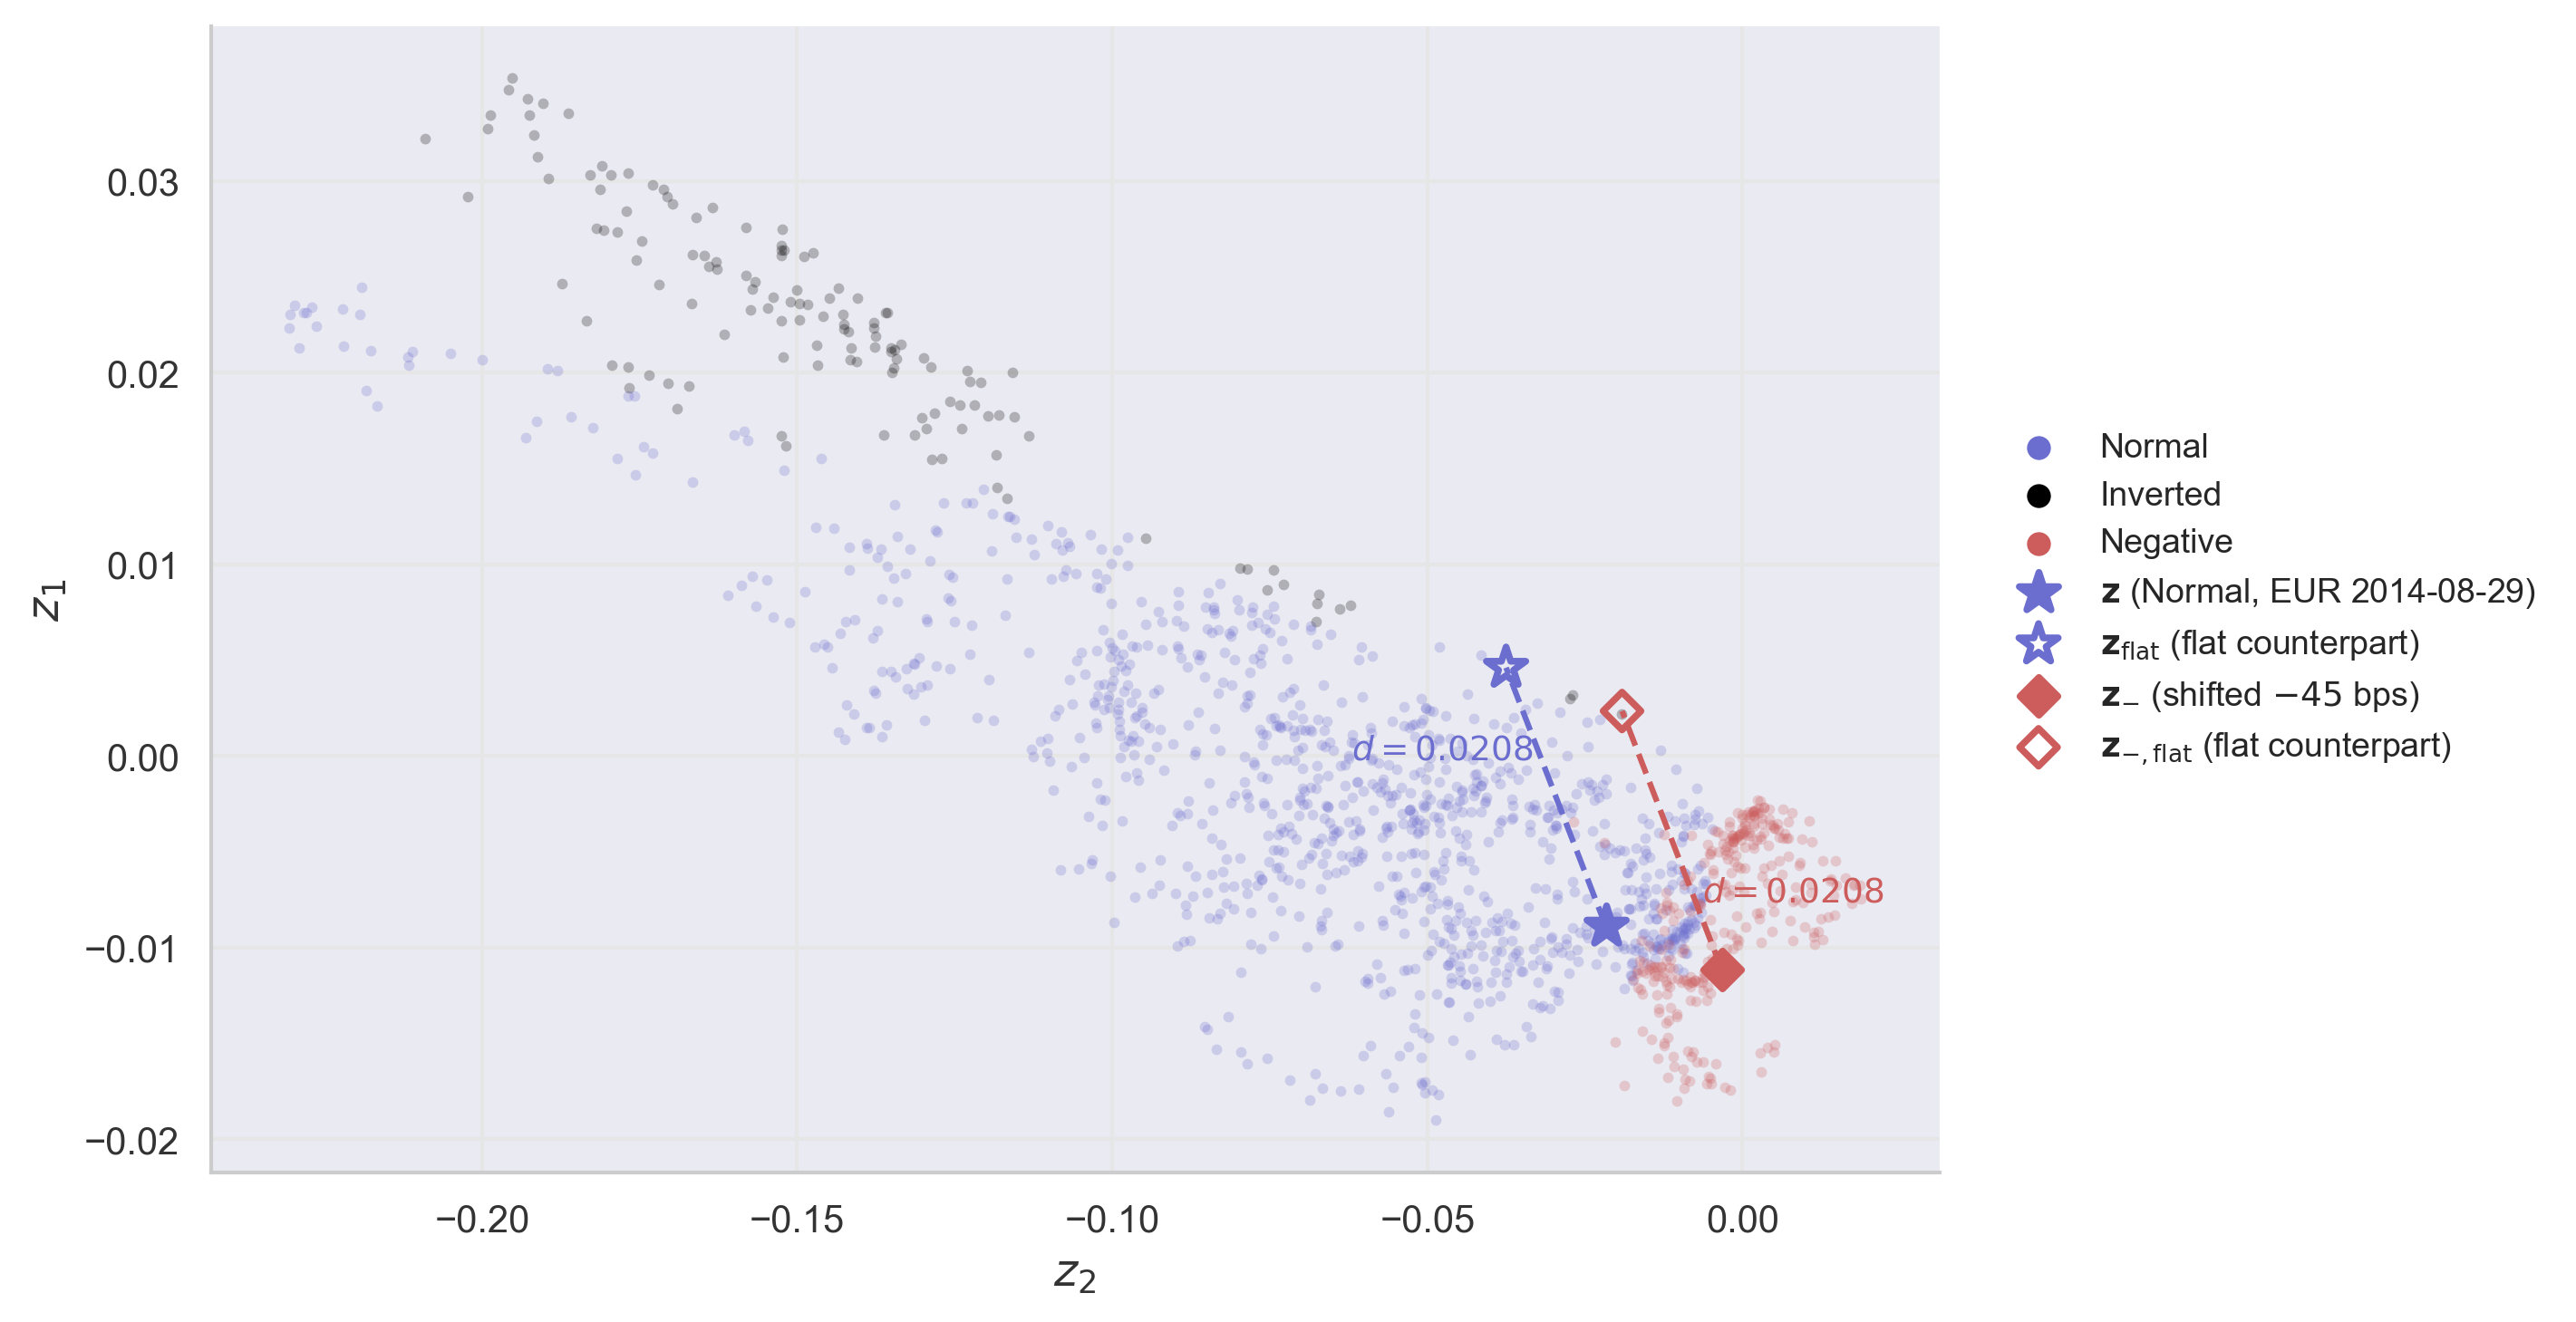
\includegraphics[width=\textwidth]{Figures/thesis_results/AutoencoderPerformanceAugmented/augmented_latent_space_regime_shift.png}
    \caption{Latent space representation of all in-sample swap rate curves under 
    the baseline encoder ($\ell = 2$), coloured by curve variant. Four specific 
    observations are overlaid: $\mathbf{z}$ and $\mathbf{z}_{\mathrm{flat}}$ 
    denote the latent representations of the normal EUR curve on 2014-08-29 and 
    its flat counterpart; $\tilde{\mathbf{z}}^-$ and $\tilde{\mathbf{z}}^-_{\mathrm{flat}}$ 
    denote the corresponding representations for the same curve shifted down by 
    45 bps. All distances are $d = 0.0208$.}
    \label{fig:latent_space_regime_shift}
\end{figure}
\end{example}

We do not formally verify this hypothesis, but use it as motivation for the 
augmentation described in the following subsection.




\subsection{Model Specification}
Motivated by this hypothesis, we augment the input vector with 
derived features. We add a short-end slope $f_1 = S_{10\text{Y}} - S_{1\text{Y}}$, a long-end slope $f_2 = S_{30\text{Y}} - S_{10\text{Y}}$, and a curvature measure $f_3 = 2S_{10\text{Y}} - S_{1\text{Y}} - S_{30\text{Y}}$. The augmented input vector is then
$$\mathbf{S}^{\text{aug}} = \bigl(S^{(1)}, \ldots, S^{(M)}, f_1, f_2, f_3\bigr)^\top \in \mathbb{R}^{M+3}$$

All three features are invariant to parallel level shifts in the rate level, meaning that replacing 
$\mathbf{S}$ by $\mathbf{S} + c\mathbf{1}$ leaves $f_1, f_2, f_3$ unchanged. For curves with \textcolor{red}{non-trivial} slope or curvature \textcolor{red}{but a low} or negative level, the derived features therefore carry shape information that the raw rates do not.  However, this argument does not apply to approximately flat curves near zero, 
where the features are themselves near zero. 


A second motivation is the training objective. Without augmentation, the loss $\lVert \mathbf{S} - \tilde{\mathbf{S}} \rVert^2$ provides no explicit incentive to match slope 
or curvature. Including the derived features in both the input and the 
loss directly penalises shape mismatch. Whether these modifications are sufficient to resolve the reconstruction failure for negative-rate curves is an empirical question, assessed in this following section.


The augmented model follows the same encoder-decoder architecture described in Chapter~\ref{chap:encoderdecodermodel}, with two modifications. The encoder receives the 11-dimensional augmented input rather than the raw 8-dimensional swap curve, and the loss is evaluated over the eight reconstructed rates plus the three derived features computed from them, giving eleven terms in total. The decoder output remains an 8-dimensional swap curve $\tilde{\mathbf{S}}$.

\subsection{Assessing the fit of Augmented}

Here we assess the in sample fit and oos of the augmented model with the baseline serving as a reference.

%We first assess whether the augmented model addresses the reconstruction failure identified for negative-rate curves. Figure~\ref{...} compares fitted and actual swap curves on the same representative dates used in Chapter~??. The baseline fit is included as a reference.


\begin{figure}[H]
    \centering
    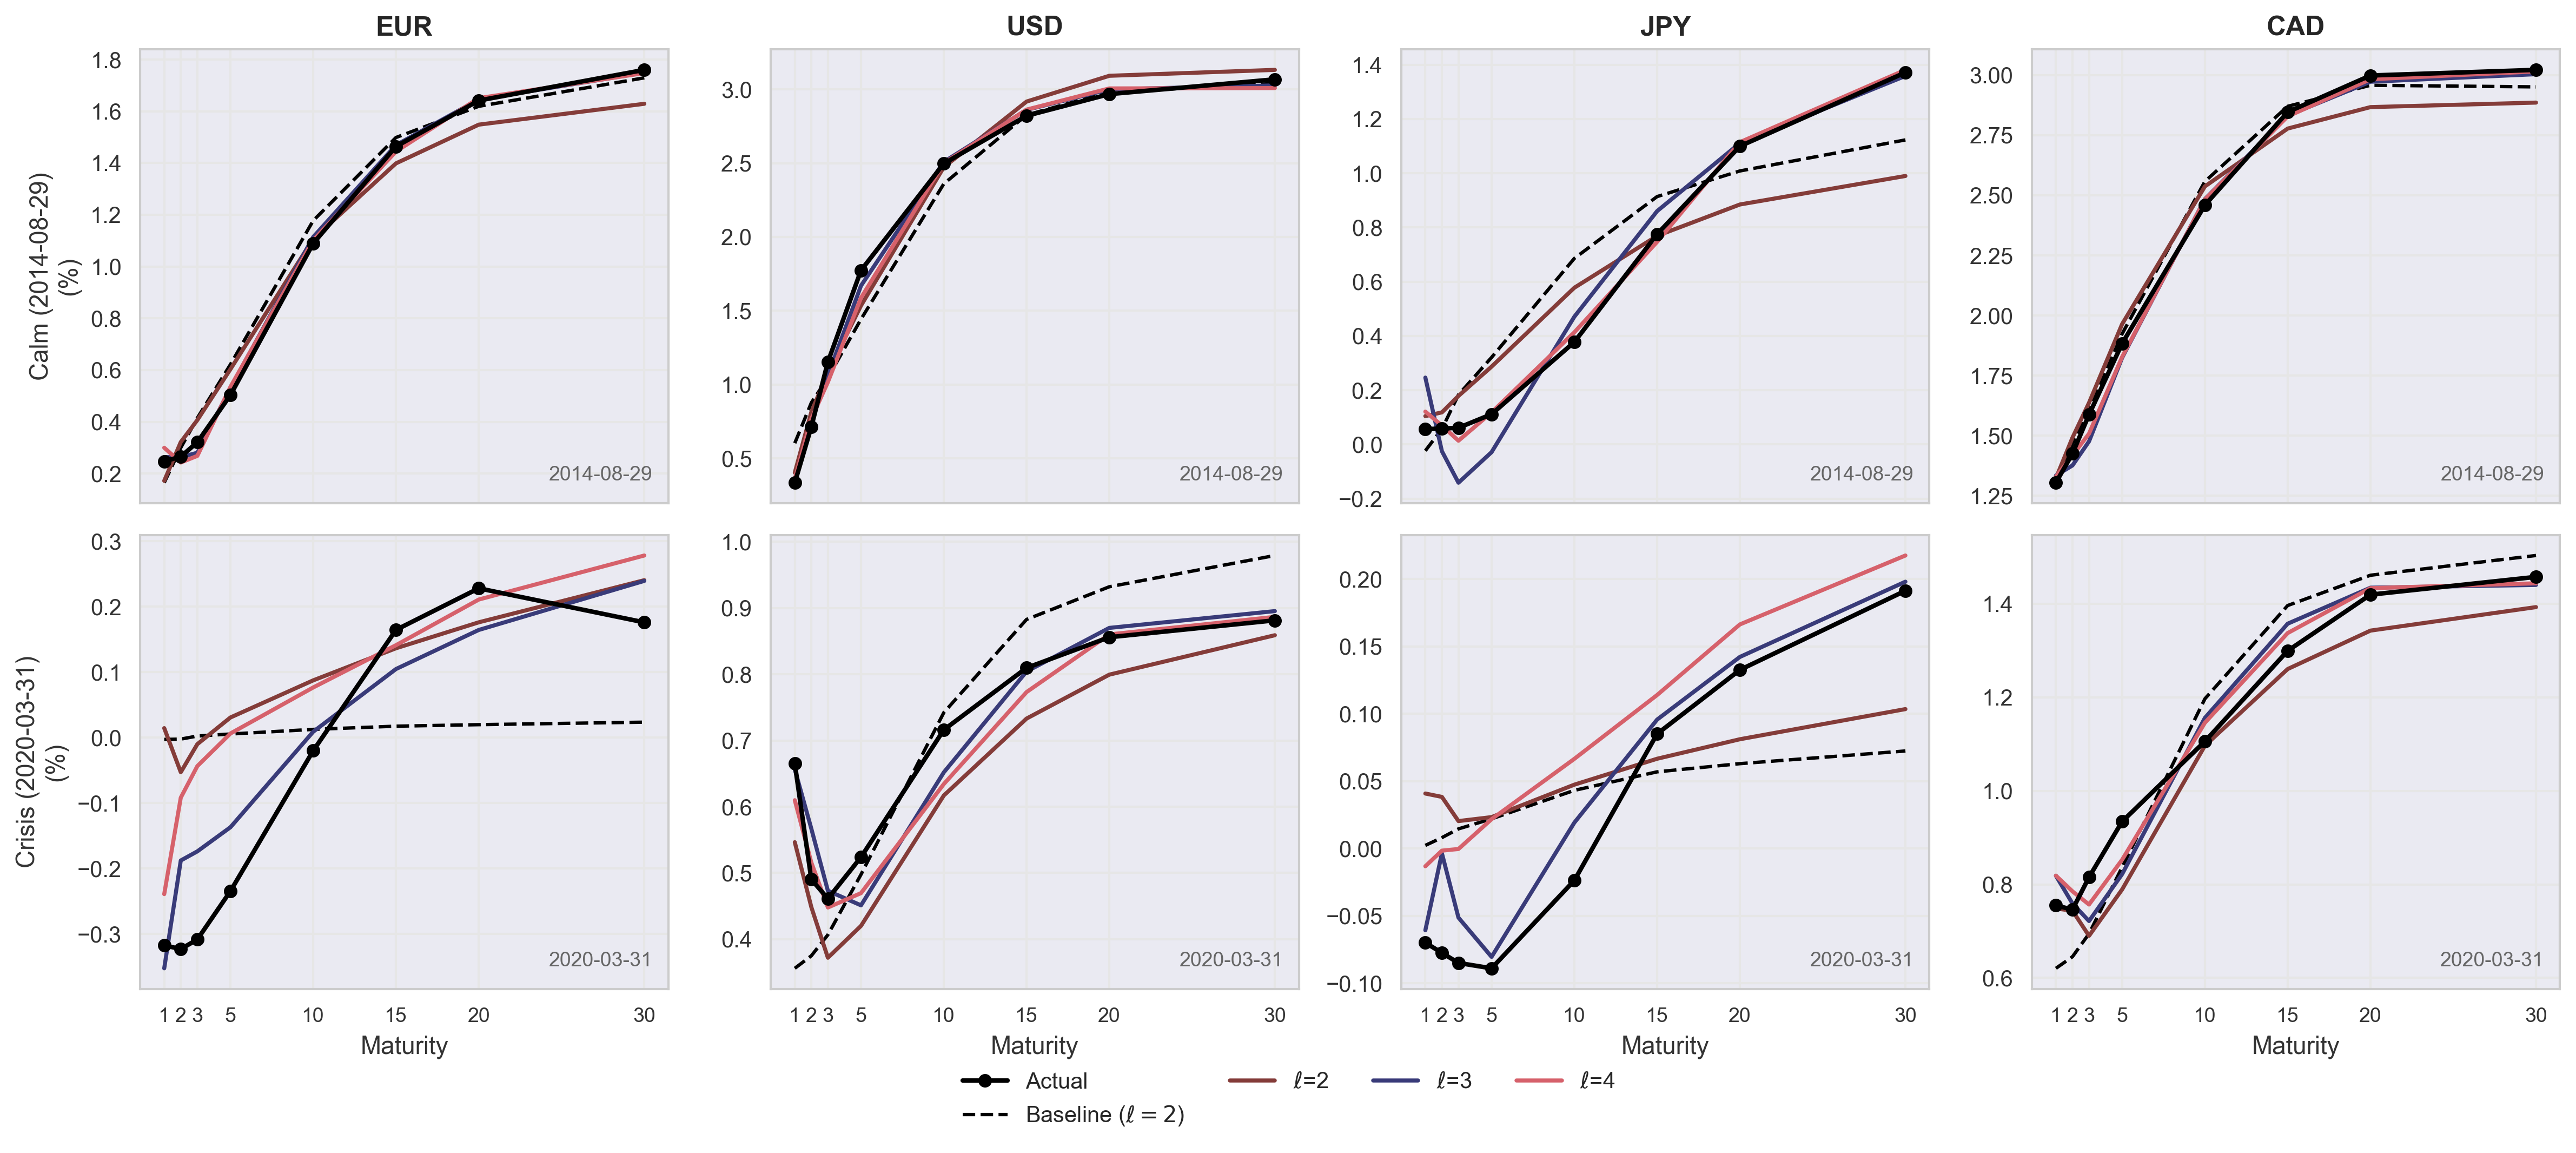
\includegraphics[width=\textwidth]{Figures/thesis_results/AutoencoderPerformanceAugmented/augmented_fitted_vs_actual_all_dims.png}
    \caption{In-sample fitted versus actual swap curves for the augmented model with
    $\ell \in \{2, 3, 4\}$ across two representative dates: a calmer market
    environment (2014-08-29) and the COVID-19 shock (2020-03-31).
    Rows correspond to market environments; columns to EUR, USD, JPY, and CAD.
    The solid line with circles denotes the observed swap rate.}
    \label{fig:augmented_fitted_vs_actual_all_dims}
\end{figure}

%The augmented model improves the in-sample fit precisely in the cases where the baseline model performed poorly. In particular, for the COVID-19 date, the fitted EUR and JPY curves reproduce more of the observed slope and curvature. This supports the interpretation that the baseline encoder did not provide the decoder with sufficient shape information in low-rate regions of the latent space.

We hereby see a great improvement in sample where the baseline had a hard time. in some way indicating that the information that we forced on the model was indeed missing for curves.

\begin{figure}[H]
    \centering
    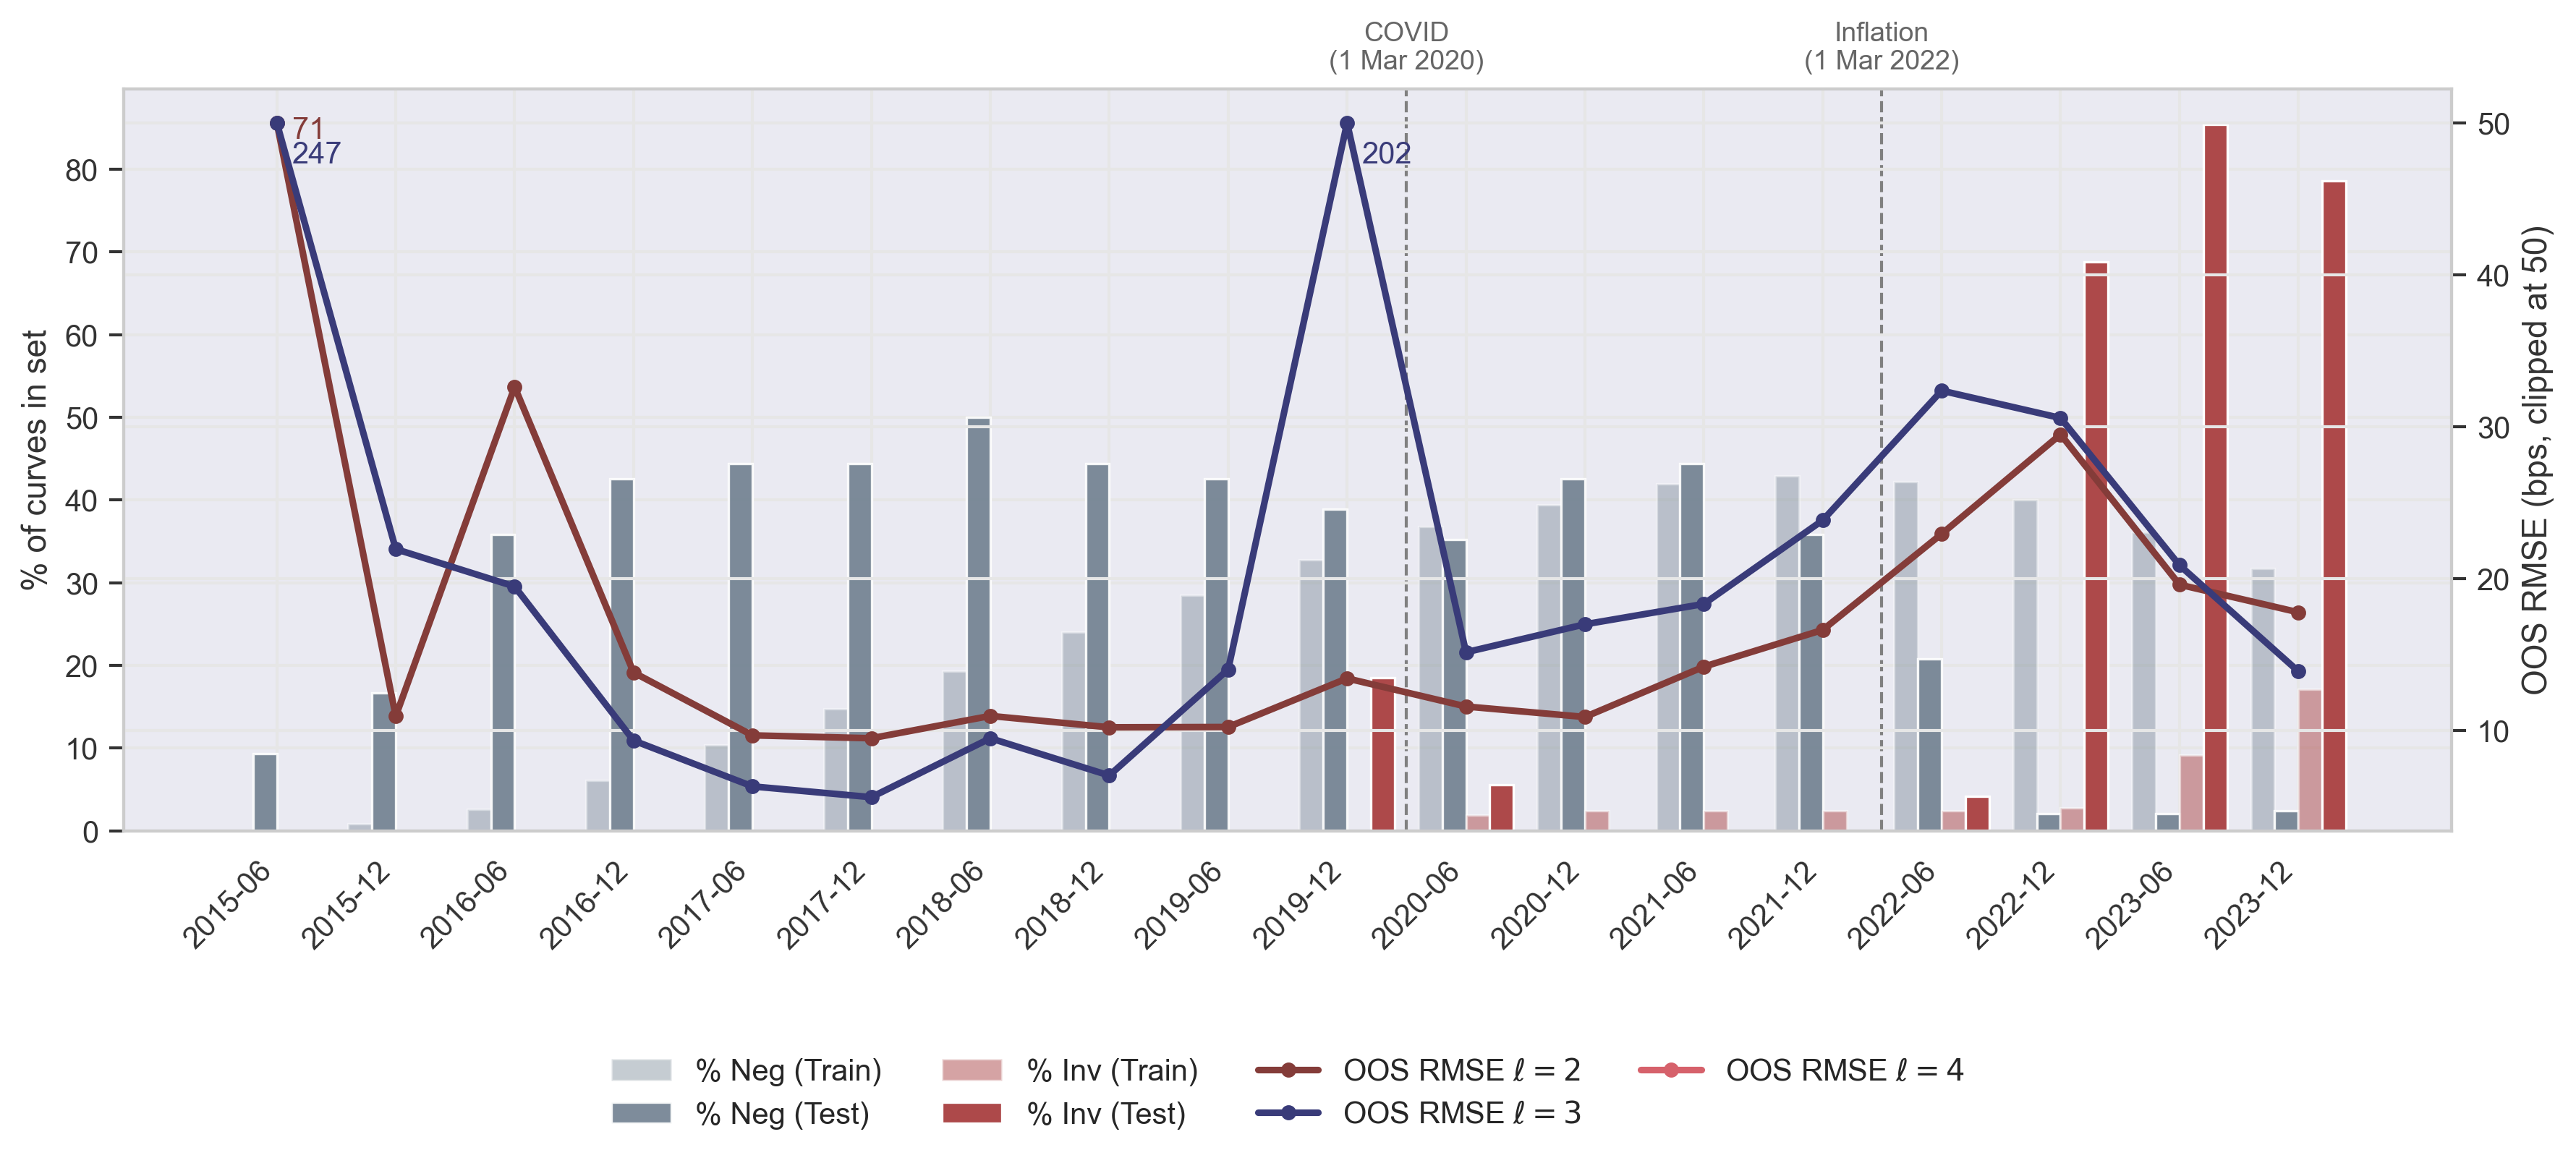
\includegraphics[width=\textwidth]{Figures/thesis_results/AutoencoderPerformanceAugmented/augmented_rolling_regime_dual_axis.png}
    \caption{Rolling out-of-sample RMSE (bps, right axis) for the augmented model
    with $\ell \in \{2, 3, 4\}$ latent factors, clipped at 50 bps for readability;
    true values are annotated where clipping occurs. Bars (left axis) show the
    percentage of curves in the negative-rate and inverted curve variants for
    the training and test set of each rolling window. Dashed vertical lines mark
    key macroeconomic events.}
    \label{fig:augmented_rolling_regime_dual_axis}
\end{figure}

%However, the improvement is mainly in-sample. The rolling-window evaluation in Figure~\ref{...} shows that the augmented model still suffers from large out-of-sample errors during periods where the test set contains curve shapes that are underrepresented in the training window.

Hereby indicating that again even with the augmented input the latent dimension 2 is the best oos even though yielding an in sample fit that was looked more like the baseline.




\section{Actual model comparison}


Combining the augmentation with the stabilisation described in Section~\ref{sec:stable} yields a fourth model, which we refer to as \textit{augmented stable}. We therefore evaluate four models in total: baseline ($\ell=3$), stable ($\ell=4$), augmented ($\ell=3$), and augmented stable ($\ell=3$). The latent dimension for each new model is selected based on its own best out-of-sample performance. 






\subsection{In-sample Fit}

In this figure below, we see how the baseline model struggles as discussed earlier with negative rate curves. And the augemnted model proposed in the section for only two dimensions does not capture this well enough. however the stable and the augmented stable models are capturing these curves relatively better, in terms of slop and curvature. IT seems as though the stbale model is better.

\begin{figure}[h]
    \centering
    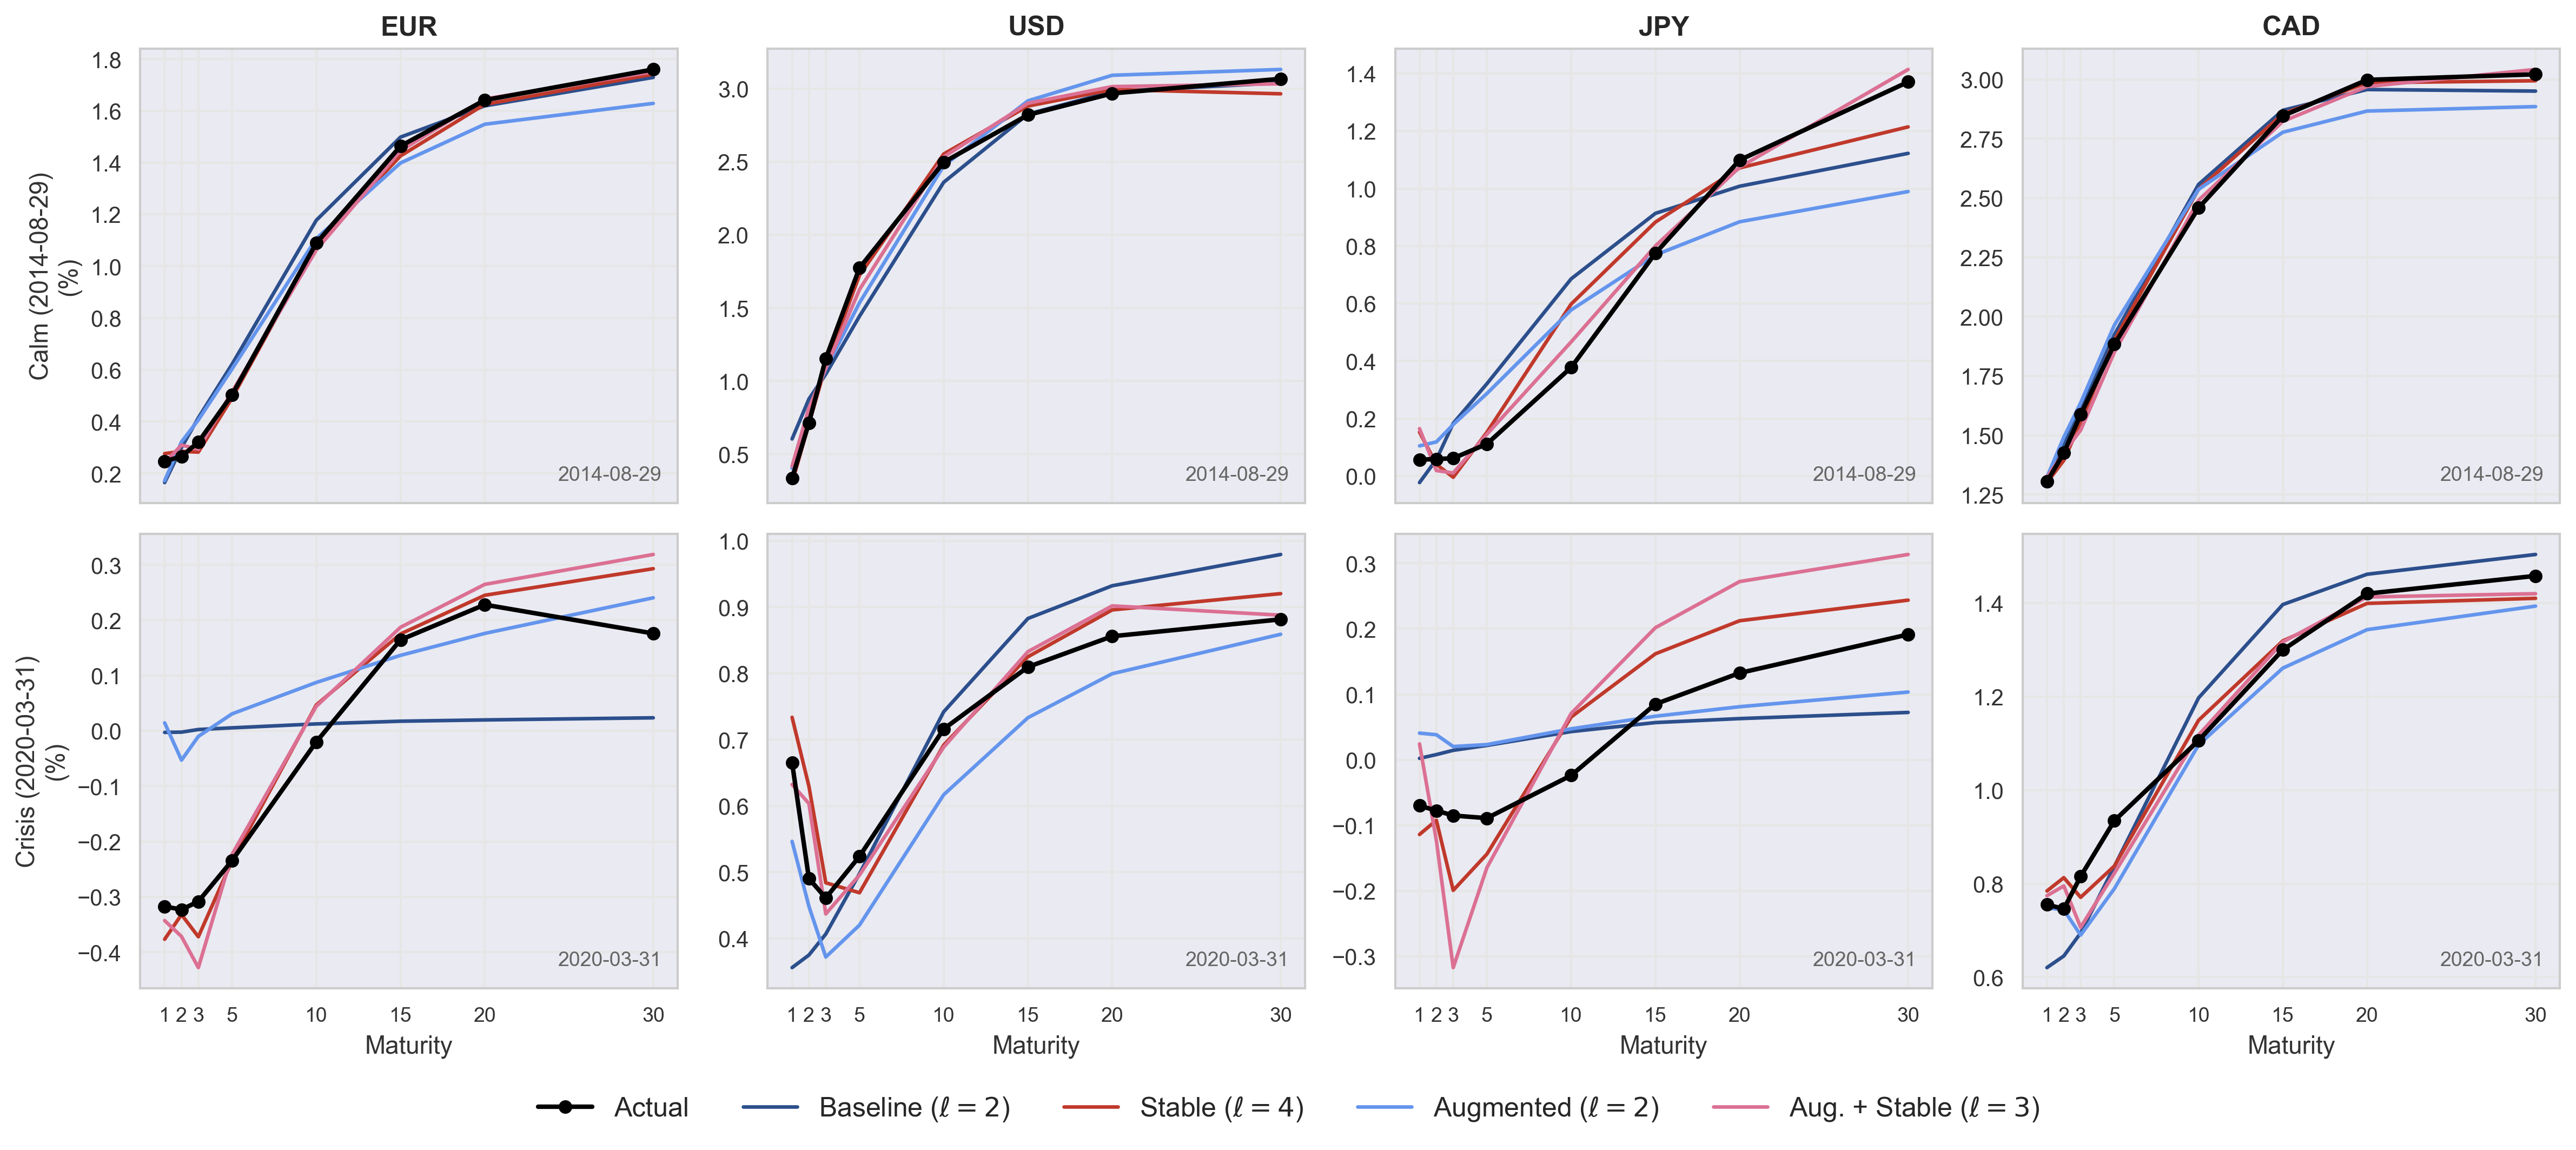
\includegraphics[width=\textwidth]{Figures/thesis_results/AutoencoderPerformanceAugmentedStable/all_models_fitted_vs_actual.png}
    \caption{Fitted versus actual swap curves for a normal market date (2014-08-29) and a crisis date (2020-03-31), shown for four selected currencies. Each panel overlays the fitted curves from the baseline ($\ell=3$), stable ($\ell=4$), augmented ($\ell=3$), and augmented stable ($\ell=3$) models.}
    \label{fig:all_models_fitted_vs_actual}
\end{figure}


\subsection{Out-of-sample Performance} 

in the oos performance we see that the stable model performs best of all four models assessed. both in terms of avereage in sample and average perfirmance. The stable model has the least generalisation gap, and most importanlty doesnt have the high explostions of max OOS SRMSE windows.

\begin{table}[H]
\centering
\pgfplotstableread[col sep=comma]{Figures/thesis_results/AutoencoderPerformanceAugmentedStable/all_models_is_oos_summary.csv}\datmodelsummary
{\footnotesize
\pgfplotstabletypeset[
  columns={Model, ell, IS_Avg, IS_Median, IS_Max, OOS_Avg, OOS_Median, OOS_Max},
  columns/Model/.style={column name={Model}, string type, column type=l},
  columns/ell/.style={column name={$\ell$}, string type, column type=c},
  columns/IS_Avg/.style={column name={Avg}, string type, column type=r},
  columns/IS_Median/.style={column name={Median}, string type, column type=r},
  columns/IS_Max/.style={column name={Max}, string type, column type=r},
  columns/OOS_Avg/.style={column name={Avg}, string type, column type=r},
  columns/OOS_Median/.style={column name={Median}, string type, column type=r},
  columns/OOS_Max/.style={column name={Max}, string type, column type=r},
  every head row/.style={
    before row={%
      \toprule
      & & \multicolumn{3}{c}{IS RMSE (bps)} & \multicolumn{3}{c}{OOS RMSE (bps)} \\
      \cmidrule(lr){3-5}\cmidrule(lr){6-8}
    },
    after row=\midrule
  },
  every last row/.style={after row=\bottomrule},
]{\datmodelsummary}
}
\caption{In-sample and out-of-sample RMSE (bps) across the four model variants. OOS results are from the rolling window evaluation scheme with 5-year training windows and 6-month test windows. The stable variant uses $\ell=4$ latent factors; all other variants use $\ell=3$.}
\label{tab:all_models_is_oos_summary}
\end{table}

However it is also important to see the error each curve as these can be easily masked in the averages. As we see here, the stable model still struggle when trained on some periods with out any  negative rates and then alot of them in the test period , with errors up to 200 for some of those curves, but this is on a much lower scale compared to the other four models. 


\begin{figure}[H]
    \centering
    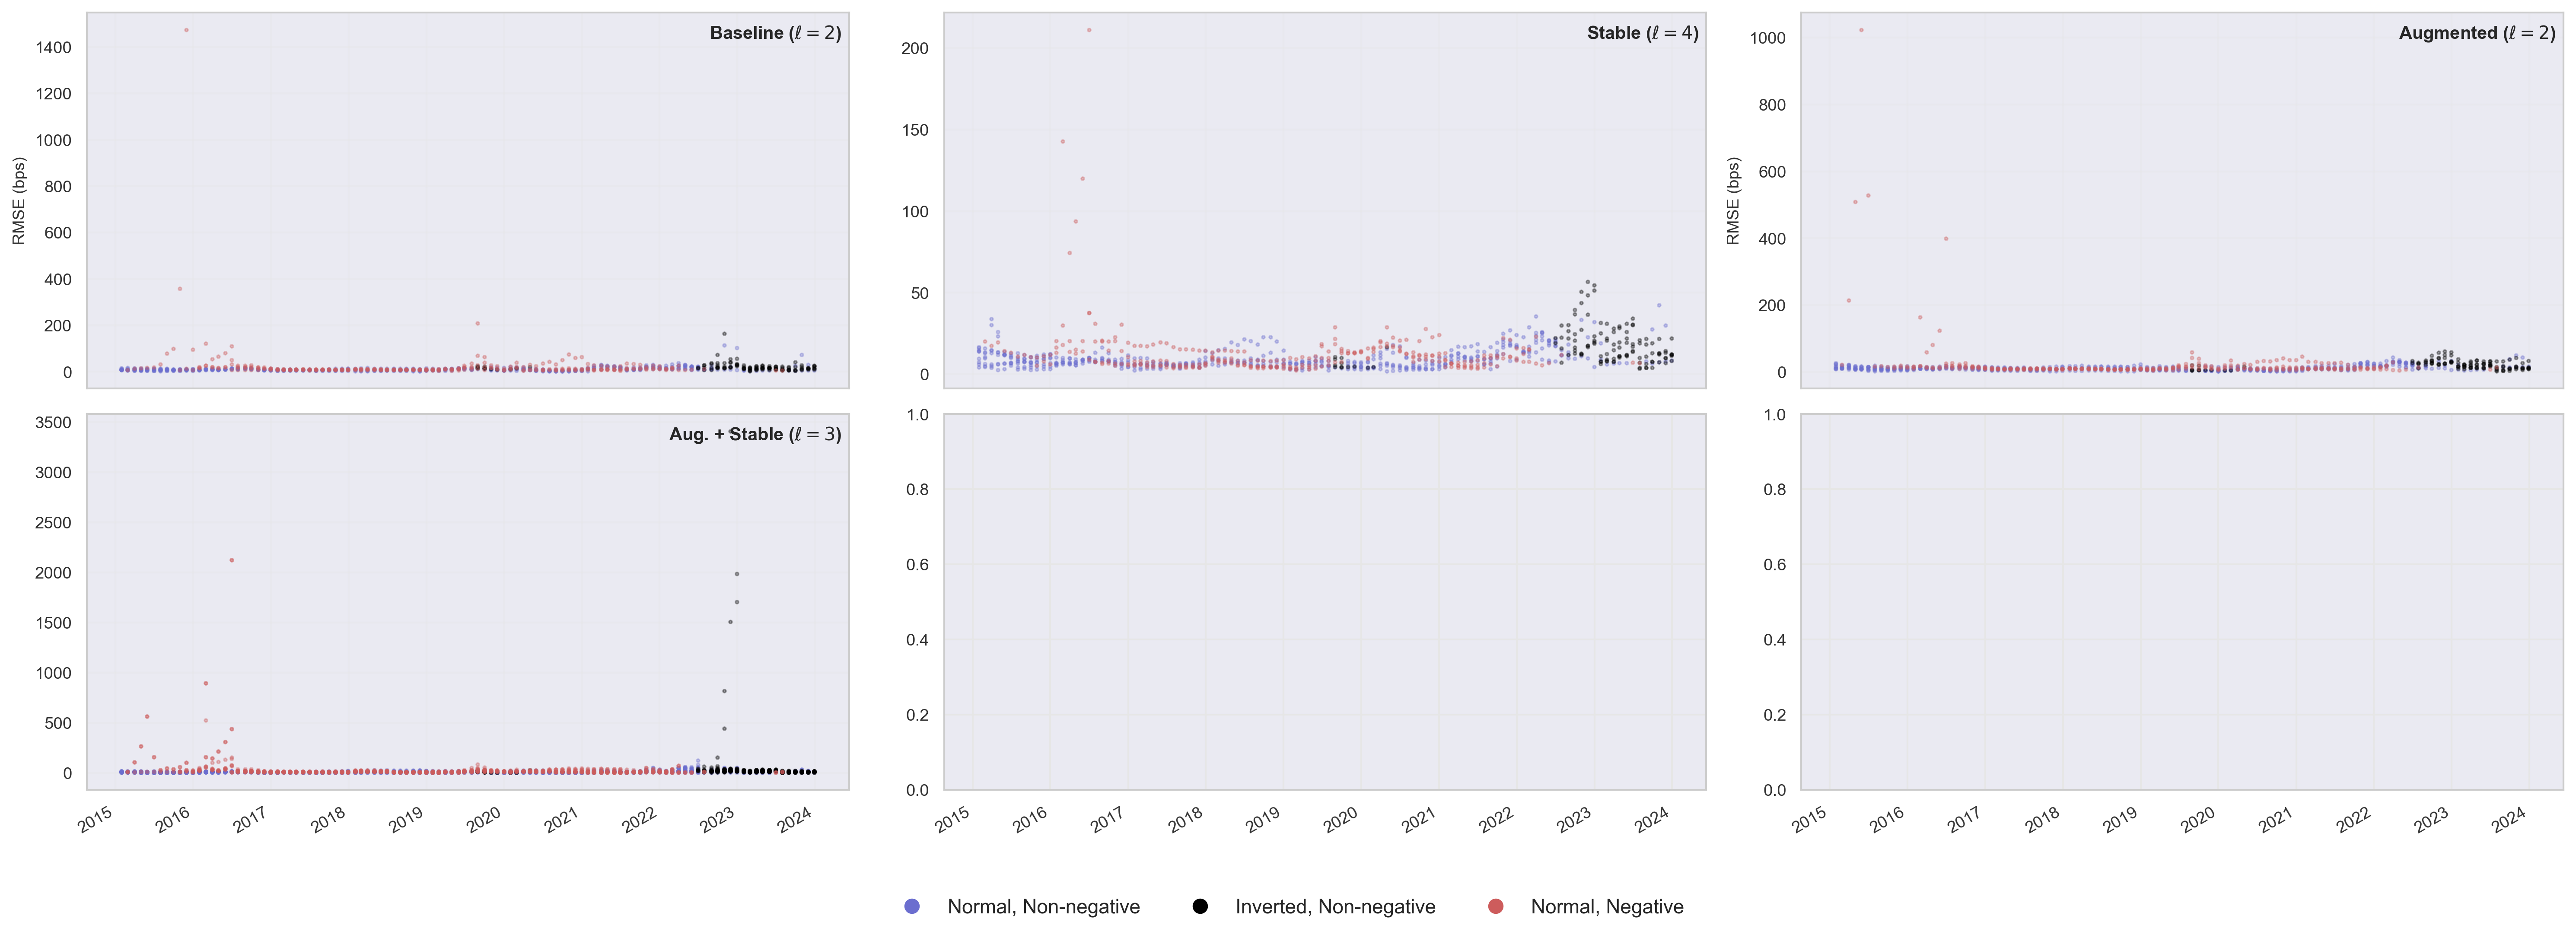
\includegraphics[width=\textwidth]{Figures/thesis_results/AutoencoderPerformanceAugmentedStable/oos_regime_scatter_all_models.png}
    \caption{Out-of-sample RMSE (bps) over the rolling evaluation period (2015--2023) for all four model variants, coloured by market regime. Each panel corresponds to one model; points are coloured by whether the curve is inverted and/or exhibits negative rates.}
    \label{fig:oos_regime_scatter_all_models}
\end{figure}

The conclusion of this is going to be about the way of how to make the encoder-decoder model to reconstruct swap curves absorb information in the best way. Baseline is completley freely, the augmented is consttraining how this is learned freely based on the training error penalizing when curves are matching on curvature and slope infromation as well, where the stable has none of these restictions in the training objective, but the neural networks have been restricted in some way so the stable model learns more effectively in some areas as so it seems. Putting these to ways of doing so together does not seem to have any positive impact, and just worsens the overeal reconstruction results.

%The comparison highlights an important distinction. The augmented model restricts learning through the reconstruction objective by forcing the model to match slope and curvature features. This improves some difficult in-sample fits, but it does not produce a more robust out-of-sample model. The stable model instead restricts the architecture of the latent dynamics and decoder. This gives the lowest average out-of-sample RMSE and, more importantly, avoids the extreme rolling-window failures observed for the other variants.

%Combining the two approaches does not improve performance. The augmented-stable model has a higher average and maximum out-of-sample error than the stable model alone. The evidence therefore suggests that, for this encoder--decoder setting, robustness is better achieved through structural restrictions on the model than through additional reconstruction penalties. The stable model is therefore the preferred specification for the pricing analysis in the next chapter.


% NOTES

%One struggle, common to both the basline model evalutaed in Chapter \ref{chap:evaluation} and the the stable model presented in Chapter \ref{chap:simulation}, is the reconstruction of curves with the negative swap rates. The baseline also had struggles with the inverted curves where the stable seem to be better in this case, but the negative rates are still the main struggle. 


%Maybe make a hypothesis that is something about the negative rates when being compressed through a linear encoder trained on non negative curves, and the used on negative rates. Like something is collapsing. SHow this in a example.

%When assessing the curve fit during the baseline evaluation, we found that the reconstructed curves of curves with negative rates found the correct level of the curve but couldnt fit the slope or the curvature well. Further the baseline also struggled with the inverted curves. The encoder-decoder models learning objective is to minimize the input swap rate curve with the reconstructed swap rate curve. We therefore propose to make it also train over more information about the curve than the mere values, there to adding three elements more to the swap rate curve input such the new input curve is:

%$$S^{\text{new}}=
%\begin{pmatrix}
%    S\\
%    S_{10}-S_1\\
%    S_{30}-S_{10}\\
%    2\cdot S_{10}-S_1-S_{30}
%\end{pmatrix}$$
%such that $S^{\text{new}}\in\mathbb{R}^m$

%Thus when training this model with this input, everything is exactly the same as explained in the Chapter \ref{chap:encoderdecodermodel}, where the three elements only are used in the part where we train the loss function, so everything is exactly the same so the encoder takes in the information and then we train the model, and as output get the recontructed $\tilde{S}$, and then from this reconstructed S calcualte the slope at the short and long end of the curve and the curvature element, and the loss function is also evaluted over these three new elements. In this way then forcing the model to also make sure to match the curve shape as well. The model that has this three new elements is denoted as augmented.

%We then train augmented together with the stable + augmented model, such that we in total have 4 different models. Since stable performed best with 4 dimeniosn and baseline best with 3, we also choose the best performing of the two new models based on their OOS performance. When assessing the curve fit trained in sample, we some very interesting results.




%From this we see that for the EUR and JPY  during the crisis dates swaprates whicg at this date have negative rates, the baseline has a very poor fit only just mathcing the level of the curve. However, in great contrast the augmented curve is clearly achieveing a better fit, now also matching the slope and curvature. The stable model despite this new  learning objective, but due to more restrictions than the baseline, also been able to handle the negative swap rate curves better. The augmented stable model seems to also find the same constructed curves as the stable bit just a bit more \textcolor{red}{volatilite} (not the right word) at then ends of the curve, suggesting...


%When assessing how the models perform OOS, they despite the better in sample fit for the harder curves to fit, still struggle despite. This is seen clearly in Tabel \ref{tab:all_models_is_oos_summary}, where there are very large errors OOS due to really bad fittings of the curves. However, we see a clear improvement insample for all models that are not the baseline model, nearly halfing the error in some cases. 











% Maybe not have enough room to showcase the short rate.

%\begin{figure}[h]
%    \centering
%    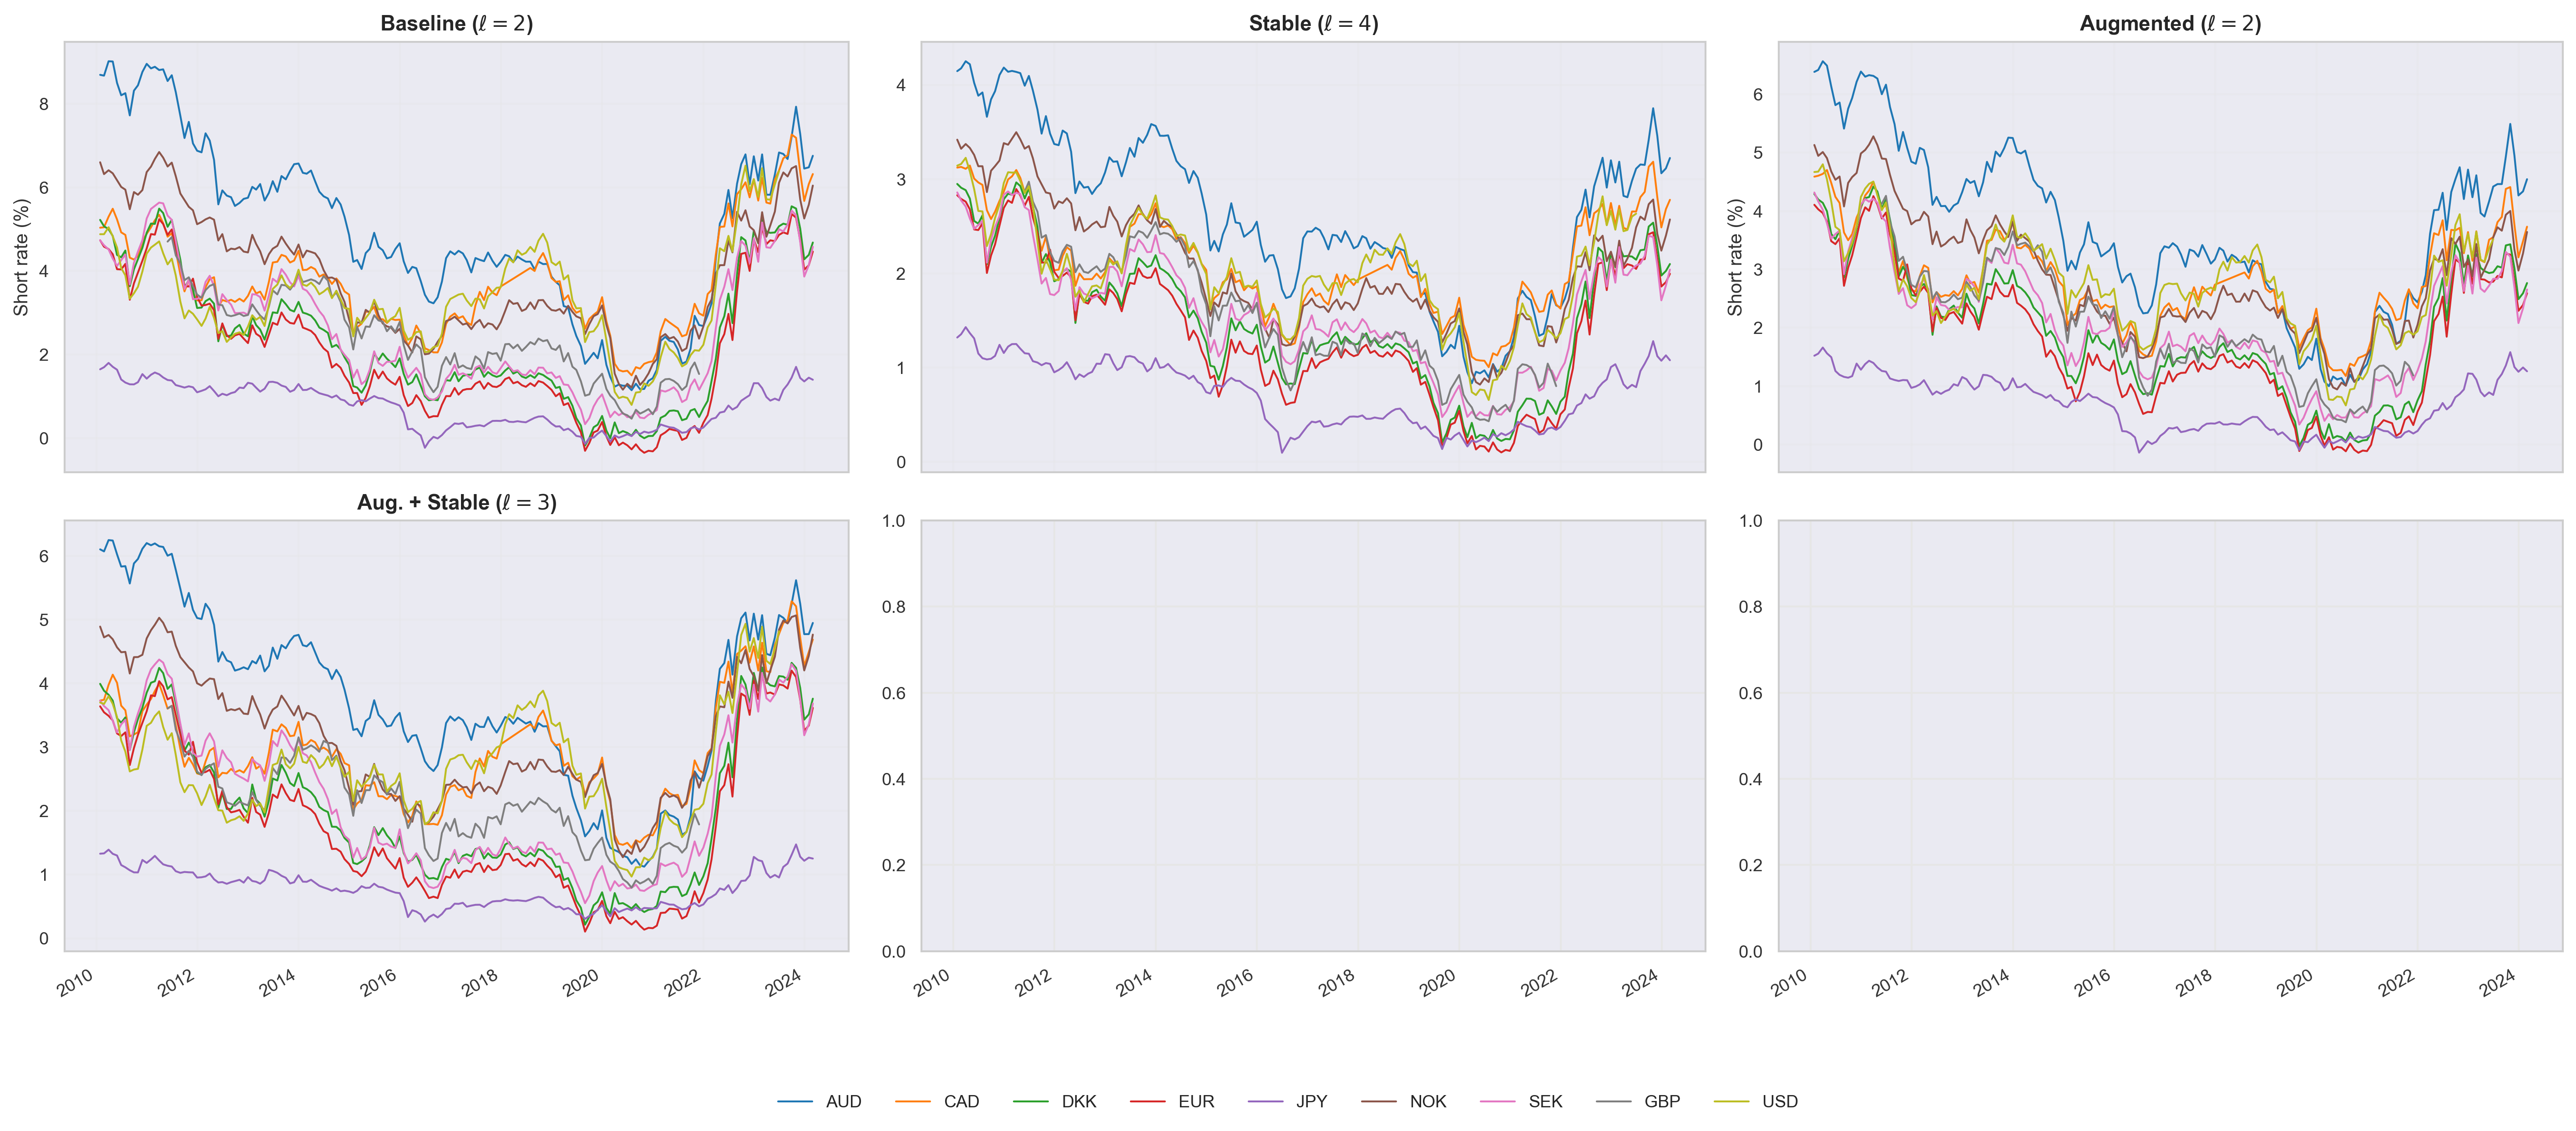
\includegraphics[width=\textwidth]{Figures/thesis_results/AutoencoderPerformanceAugmentedStable/all_models_short_rate.png}
%    \caption{X}
%    \label{fig:all_models_short_rate}
%\end{figure}
